\documentclass[10pt,a4paper]{article}
\usepackage[latin1]{inputenc}
\usepackage{amsmath}
\usepackage{amsfonts}
\usepackage{amssymb}
\usepackage{fullpage}
\usepackage{graphicx}

\usepackage{multicol}

\begin{document}
\title{Goldstein, Poole, and Safko Problem 1.19}
\author{Josh Orndorff \\ admin@joshorndorff.com}
\maketitle

\begin{figure}[hbtp]
\caption{Spherical pendulum with coordinates labelled}
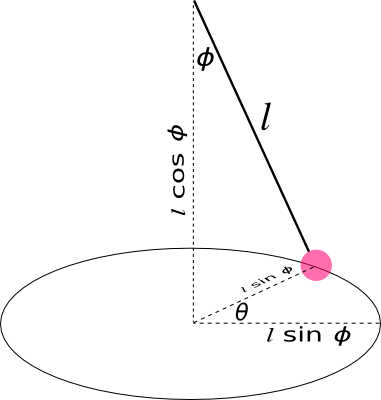
\includegraphics[scale=.6]{Goldstein1-19.png}
\end{figure}


Establishing the coordinate system as it is labelled in the figure, we can begin by writing the potential and kinetic energy functions.

\begin{equation}
U=-mgl\cos\phi
\end{equation}
\begin{equation}
T= \frac{1}{2}m\left(l^2\dot{\theta}^2 \sin^2\phi +l^2\dot{\phi}^2\right)
\end{equation}
\begin{equation}
T= \frac{ml^2}{2}\left(\dot{\theta}^2 \sin^2\phi +\dot{\phi}^2\right)
\end{equation}

That being established,we can write the Lagrangian as $L=T-U$.
\begin{equation}
L= \frac{ml^2}{2}\left(\dot{\theta}^2 \sin^2\phi +\dot{\phi}^2\right) + mgl\cos\phi
\end{equation}

Now that we have the Lagrangian in all of its glory, we can compute the appropriate derivatives that we will need to find the equations of motion.

\begin{table}[h]
\centering
\begin{tabular}{ll}
$\frac{\partial L}{\partial \theta}= 0$ &
$\frac{\partial L}{\partial \phi}=ml^2\dot{\theta}^2\sin\phi\cos\phi$\\
$\frac{\partial L}{\partial \dot{\theta}}=ml^2\dot{\theta} \sin^2\phi$ &
$\frac{d}{dt}\frac{\partial L}{\partial \dot{\phi}}=ml^2\dot{\phi}$\\
$\frac{d}{dt}\frac{\partial L}{\partial \dot{\theta}}=ml^2 \left(\ddot{\theta}\sin^2\phi+2\dot{\theta}\dot{\phi}\sin\phi\right)$&
$\frac{d}{dt}\frac{\partial L}{\partial \dot{\phi}}=ml^2\ddot{\phi}$\\
\end{tabular}
\end{table}

Now we can use the Euler Lagrange equation to determine the equations of motion.  The $\phi$ equation becomes:
\begin{equation}
ml^2\dot{\theta}^2 \sin\phi\cos\phi-mgl\sin\phi=ml^2\ddot{\phi}
\end{equation}
\begin{equation}
\ddot{\phi}-\dot{\theta}^2\sin\phi\cos\phi+\frac{g}{l}\sin\phi=0
\end{equation}

The Euler Lagrange equation for $/theta$ is:
\begin{equation}
ml^2 \left(\ddot{\theta}\sin^2\phi+2\dot{\theta}\dot{\phi}\sin\phi\right)=0
\end{equation}
What this really tells us is that the quantity $\frac{\partial L}{\partial\dot{\theta}}$ is conserved.

These equations are not solvable analytically, but could be solved numerically.
\end{document}